\documentclass[a4paper,11pt]{article}
\usepackage{amsmath}
\usepackage{graphicx}
\usepackage{float}
\usepackage[utf8]{inputenc}

\title{MaS Assignment II\\
\large Percolation}
\author{Klaas Kliffen s2369494}
\date{\today}

\begin{document}

\maketitle

\section{Introduction}
The percolation model can be seen as a extremely simple randomised growth model without particle diffusion.
At each step, for all available unmarked neighbour sites to an existing cluster, each one is marked occupied with a fixed probability $p$ or empty with probability $1-p$. Only unmarked sites may be occupied. The probability is the only parameter of this model.

\subsection{Initialisation}
This assignment considers a percolation growth on a square lattice with a fixed size of ($2N+1\times(2N+1)$. The clusters starts at the center of the lattice at $(N,N)$, the rest of the lattice remains unmarked.

\subsection{Stopping conditions}
The model stops when either (a) all neighbour sites of a cluster are marked empty or (b) the cluster ahas reached the border of the lattice, i.e. any site in row or column number 1 or $2N+1$ is occupied.\\
Case (a) refers to a non-percolating or finite cluster. Case (b) is called a percolating or infinite cluster.

\subsection{Cluster size statistics}
The first core problem will focus on statistics on the size of generated clusters and whether they are finite or infinite.\\

\subsection{System size dependence}
The size of the lattice may influence the growth of clusters and the number of clusters becoming percolating.

\section{Methods}
This section globally describes the parameters used for this assignment.
\subsection{Cluster size statistics}
For each probability 100 runs will be used to calculate the mean and standard deviation on the size of a cluster. Only non percolating clusters will be used in the statistics, since the size of the cluster for percolating clusters is not defined.
The clusters will be generated on a lattice of size 99 by 99 sites. Values of $p$ in the range of [0.3,0.7] will be used. Values for either smaller than 0.3 or larger than 0.7 will be neglected. Either the value of $p$ will be too small and not generate a cluster or if $p$ is too large, all clusters will reach the boundary. A step size for $p$ of 0.05 is used.\\

\subsection{System size dependence}
The system size dependence uses the same method as with the cluster size statistics, only using different size for the lattice. The sizes used for the lattices are: $11\times11$,$21\times21$ and $41\times41$

\section{Results}
\subsection{Cluster size statistics}
\begin{figure}[H]
\centering
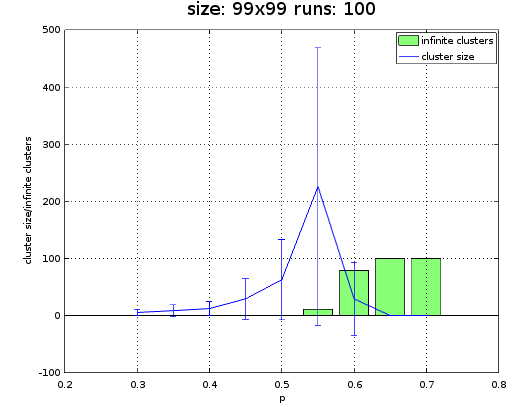
\includegraphics[width=\textwidth]{img/s99r100.png}
\caption{100 runs on a 99 by 99 lattice with $p$ in [0.3,0.7]}
\label{s99}
\end{figure}
In figure \ref{s99} the blue line represent the mean cluster size for a given $p$ with error bars showing the standard deviation. The green bars represent the number of runs which yielded a percolating cluster.\\
The mean cluster size increases until $p = 0.55$. Above that probability the mean cluster size will decrease, due to there being more percolating clusters.
An interesting fact can be seen that until $p = 0.55$ the standard deviation increases. The standard deviation at $p = 0.5$ and $p = 0.55$ is larger than the mean cluster size. This indicates a large spread of cluster sizes, either being very large or very small.\\
The number of infinite clusters slowly increases after $p = 0.55$ reaching 100 for the higher values for $p$. Since the number of runs was 100, this fraction will be 1.
This means that after $p = 0.55$ it becomes more probably for a cluster to be percolating than being a finite cluster.

\subsection{System size dependence}
\begin{figure}[H]
\centering
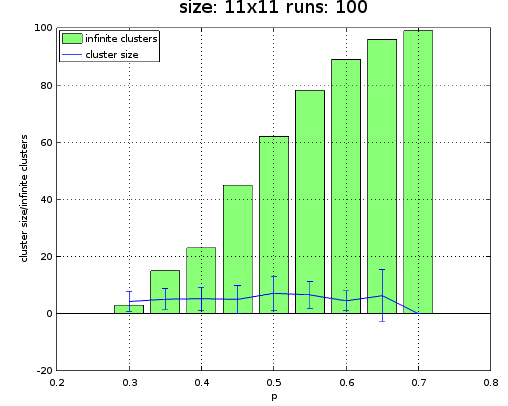
\includegraphics[width=.8\textwidth]{img/s11r100.png}
\caption{100 runs on a 11 by 11 lattice with $p$ in [0.3,0.7]}
\label{s11}
\end{figure}
\begin{figure}[H]
\centering
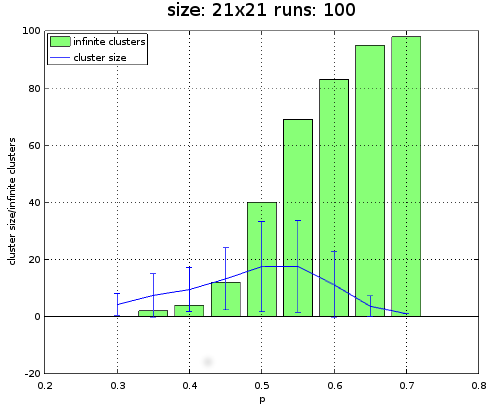
\includegraphics[width=.8\textwidth]{img/s21r100.png}
\caption{100 runs on a 21 by 21 lattice with $p$ in [0.3,0.7]}
\label{s21}
\end{figure}
\begin{figure}[H]
\centering
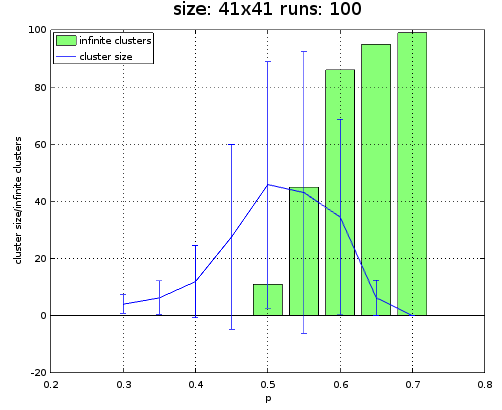
\includegraphics[width=.8\textwidth]{img/s41r100.png}
\caption{100 runs on a 41 by 41 lattice with $p$ in [0.3,0.7]}
\label{s41}
\end{figure}
Comparing the cluster size and fraction of percolating cluster for different lattice sizes for the values of $p = 0.3$ and $p = 0.7$ yields similar values for cluster size and fraction of percolating clusters for all lattice sizes.\\
A difference between the size can be seen at which value for $p$ the fraction of percolating cluster starts to emerge. In figure \ref{s11} this start even at the lowest value of $p = 0.3$. Also, the increase seems to be almost linear for increasing the value of $p$. While in figures \ref{s21},\ref{s41} and also in figure \ref{s99} seems to be more like a inverse tangent function with a translation to the right. The probability $p$ at which the percolating start to appear, increases with the lattice size. 
For an infinite lattice, the fraction would only start to appear at $p=1$. As there are an infinite amount of neighbour sites with a probability for each one to be empty, eventually stopping the cluster to grow.\\
Another difference can be seen at the probability $p=0.5$. Increasing the size of the lattice also increases the mean cluster size and the standard deviation of cluster sizes.

\section{Conclusion and discussion}
\subsection{Cluster size statistics}
The mean cluster size grows exponentially with $p$. The cluster sizes however are very skewed for very large and very small clusters, with a large standard deviation.
The fraction of percolating clusters also increases with $p$. Only starting at $p=0.55$ for a lattice with size $99\times99$.
\subsection{System size dependence}
The model seems to be dependent on the size of the lattice. For $p = 0.3$  and $p = 0.7$ the values for the mean cluster size and number of percolating clusters might be similar. But for values in between these statistics do differ.\\
Another observation is at which value for $p$ the percolating clusters start to appear, increasing with the cluster size. Eventually becoming $p = 1$ for an infinite lattice.
\subsection{Discussion}
In this assignment the cluster always started at the center point of the lattice. A cluster started at a random point in the lattice might yield different results. Especially if the point is chosen near one of the borders, the number of percolating clusters might increase.

\end{document}
